\documentclass[11pt, a4paper, oneside]{report}
% \usepackage[left=2cm, right=2cm, top=1.5cm, bottom=1.5cm]{geometry}

\usepackage{float} % lets you have non-floating floats
\usepackage{url} % for typesetting urls

\usepackage{amsmath}

\usepackage{hyperref}
\usepackage{cleveref}

\usepackage{wrapfig}
\usepackage{subcaption}
\usepackage{graphicx}
\usepackage[table,xcdraw]{xcolor}

\usepackage{pdfpages}

\definecolor{mGreen}{rgb}{0,0.6,0}
\definecolor{mGray}{rgb}{0.5,0.5,0.5}
\definecolor{mPurple}{rgb}{0.58,0,0.82}
\definecolor{backgroundColour}{rgb}{0.95,0.95,0.92}

% Include C code
\usepackage{listings}
\lstset{
  backgroundcolor=\color{backgroundColour},   
  commentstyle=\color{mGreen},
  keywordstyle=\color{magenta},
  numberstyle=\tiny\color{mGray},
  stringstyle=\color{mPurple},
  basicstyle=\ttfamily\small,
  columns=flexible,
  keepspaces=true,
  language=C,                     % choose the language of the code
  numbers=left,                   % where to put the line-numbers
  stepnumber=1,                   % the step between two line-numbers.        
  numbersep=5pt,                  % how far the line-numbers are from the code
  backgroundcolor=\color{white},  % choose the background color. You must add \usepackage{color}
  showspaces=false,               % show spaces adding particular underscores
  showstringspaces=false,         % underline spaces within strings
  showtabs=false,                 % show tabs within strings adding particular underscores
  tabsize=2,                      % sets default tabsize to 2 spaces
  captionpos=b,                   % sets the caption-position to bottom
  breaklines=true,                % sets automatic line breaking
  breakatwhitespace=true,         % sets if automatic breaks should only happen at whitespace
  title=\lstname,                 % show the filename of files included with \lstinputlisting;
  emph={%  
    uint8_t, uint16_t, uint32_t, TaskHandle_t, QueueHandle_t, esp_adc, esp_err_t, PIDController, ledc_timer_config_t, ledc_channel_config_t, TickType_t%
    },emphstyle=\color{magenta},
}

% Make the title spacing smaller
% \usepackage{titlesec}
% \titleformat{\chapter}[hang] 
% {\normalfont\huge\bfseries}{\chaptertitlename\ \thechapter:}{1em}{} 
% \titlespacing*{\chapter}{0pt}{-50pt}{40pt}

\newcommand{\todo}[1]{\textcolor{red}{#1}}

\hypersetup{
    colorlinks=true,
    linkcolor=black,
    filecolor=black,
    citecolor=black,
    urlcolor=black,
}

\usepackage[image,ecs]{vuwproject}

% \renewcommand{\thesection}{\arabic{section}}
% \setlength{\parskip}{\baselineskip}
\setlength{\parindent}{0pt}

\usepackage{titlesec}
\titleformat{\chapter}[hang] 
{\normalfont\huge\bfseries}{\chaptertitlename\ \thechapter:}{1em}{} 

%
%  We don't want figures to float so we define
%
\newfloat{fig}{thp}{lof}[chapter]
\floatname{fig}{Figure}
\graphicspath{ {./Figures/} }

%% These are standard LaTeX definitions for the document
%%                            
\title{Self Tuning Buck Converter}
\author{Niels Clayton}

\supervisors{Daniel Burmester and Ramesh Rayudu}
\otherdegree{Bachelor of Engineering with Honours}

\date{}

\begin{document}

\frontmatter

%%%%%%%%%%%%%%%%%%%%%%%%%%%%%%%%%%%%%%%%%%%%%%%%%%%%%%%

\begin{abstract}

    Switch-mode power supplies are commonly used in a wide variety of consumer and professional appliances to transform DC voltages with high efficiency. One such switch-mode supply is the buck converter, which steps down a DC voltage. The current buck converter design process requires that a specific output filter be designed around the switching frequency of the converter, the required output voltage, and the desired inductor ripple. This filter design process often results in the selection of non-standard components that are difficult to purchase or manufacture, increasing costs and leading to design compromises. This project will develop a platform that allows for observation and control of the inductor current ripple by modulating the switching frequency of the converter. This will allow engineers to design buck converters directly for the specified inductor current ripple their application can tolerate, eliminating the issues of designing this output filter.

\end{abstract}

%%%%%%%%%%%%%%%%%%%%%%%%%%%%%%%%%%%%%%%%%%%%%%%%%%%%%%%

\maketitle

\setcounter{tocdepth}{1}
\tableofcontents
% \listoffigures
% \listoftables

%%%%%%%%%%%%%%%%%%%%%%%%%%%%%%%%%%%%%%%%%%%%%%%%%%%%%%%

\mainmatter

%%%%%%%%%%%%%%%%%%%%%%%%%%%%%%%%%%%%%%%%%%%%%%%%%%%%%%%

% individual chapters included here
\chapter{Introduction}\label{C:intro}

Historically power distribution has been primarily in the form of AC (Alternating current). This is credited to the fact that AC power is more efficient to transmit over long distances and made it easy to step up and down the voltages efficiently with transformers \cite{Earley2013}. However, with the invention of solid-state electronics such as the metal–oxide–semiconductor field-effect transistor or MOSFET for short, it has become possible to efficiently step up and step down direct current (DC) voltages. This has been achieved by the invention of the switch-mode power supply, which has facilitated the continued reduction of size and increase in efficiency of electronics \cite{Bocock}.

Today, switch-mode power supplies can be found in a wide variety of consumer and professional electronics, with some examples being laptops, phones, and any form of DC charger. Their widespread usage when compared to other DC-DC converters such as linear regulators can be attributed to their far greater efficiency. One such switch-mode power supply is the buck converter, which will step down a DC input voltage to a lower DC output voltage.

\section{Project Motivation}

Although buck converters are a widespread technology, they are not without their limitations and drawbacks. The current buck converter design process requires that a specific output filter be designed around the switching frequency of the converter, and the desired inductor ripple. This filter design process will often result in the converter requiring discrete passive components that are non-standard and hard to source. This will usually result in the designer having to make compromises in their design for either the cost or the performance of the converter.

Another drawback of this design process is the static nature of both the filter and the switching components once they have been selected. This results in the buck converters desired inductor current ripple only being achieved at a very specific designed output voltage or load. This means that with current buck converter designs varying the desired output voltage or varying the output load will cause the inductor current ripple to vary. This is an issue, as very few loads are static and will not change during their operation. 

\section{Project Goals}

This project aims to eliminate the need to design the output stage of a buck converter. By implementing a control system that varies the switching frequency of the converter, we will be able to directly manipulate the inductor current ripple. This project aims to produce a proof of concept buck converter that is capable of operating at 12V, with an output range of 3-10V and precision of $\pm5\%$. The converter will also be able vary its switching frequency between 1$kHz$ and 100$kHz$, allowing for selection of inductor current ripple between 20\% and 50\% with precision of $\pm5\%$. All of this must be implemented while maintaining the standard functionality of the converter. For full system requirements please refer to \Cref{A:proposal}.

\subsubsection{TODO Expand on the project goals, possibly convert the previous section into a bulleted list of project goals and requirements.}

This will be referenced in the implementation and design sections many times, so it needs to clearly outline what we are looking to achieve in this project. 
\chapter{Background}\label{C:background}

A literature research was performed to inform design decision made in this project, and to evaluate any existing research. It will discuss buck converter design factors and topologies, as well as the various different methods of PWM generation. In performing this literature research, the following terms were used to search for articles from Google Scholar, Engineering Village, and Te Waharoa:

\begin{itemize}
    \item Frequency Variable PWM
    \item Frequency-PWM converter
    \item Switching Frequency Converter
\end{itemize}

These searches returned no research relevant to the designs of this project, with the only related work focusing on the electromagnetic noise reduction using randomised frequency modulation \cite{Roman2001,Familiant2016}. Because of this, research was instead performed to inform the design of the buck converter and the generation of PWM signals.

\section{PWM Generation}\label{S:PWM}

\begin{itemize}

    \item
          Discuss what PWM is, and how it is used in the context of a buck converter.

    \item
          Discuss the different methods of PWM generation.

          \begin{itemize}
              \item Analogue
              \item Digital (Microcontroller \& FPGA)
          \end{itemize}

    \item
          Discuss how PWM is used in the context of the project. Quickly overview how in this project it will be important to modulate both the PWM frequency, and the PWM duty cycle.

\end{itemize}


\section{Buck Converters}\label{S:buck}

The buck converters is a variant of a switch mode power supply that steps down a DC input voltage to a DC output voltage. They are commonly used in a wide variety of consumer and professional appliances such as laptops, phones, and chargers due to their high efficiency compared to other DC-to-DC step down converters such as linear regulators \cite{Mohan2012}.\\

The basic operational components of a buck converter can be seen below in Figure \ref{F:buck_func}. From this we see that a buck converter has three main elements, the input voltage source, two switching components, and an output filter across the load. In the case of Figure \ref{F:buck_func}, the first switching component is an actively controlled switch such as a MOSFET or transistor, and the second a passive switching diode. This configuration of an active and a passive switch is known as the non-synchronous buck converter topology, if the passive diode were to be replaced with a second active switch the topology would be considered synchronous. Although both topologies function under the same fundamental principles, the non-synchronous topology is easier to implement with the drawback of higher losses and therefor lower efficiency.\\

It can also be seen from Figure \ref{F:buck_func} that a buck converter has two operating states that are controlled through the activation of these switching components. By toggling these switching components at high speed though the use of PWM, we can control the current flowing through the inductor of the output filter. By controlling this current we are also able to directly control the current through, and voltage across the output load of the converter. Using this, buck converters will often have a feedback control system in their design to be able to actively control and regulate the output voltage during usage. This controller will vary the duty cycle of the the switching PWM signal, thereby varying the output voltage of the buck converter as shown in Equation \ref{E:V_out}\\

\begin{figure}[H]
      \includegraphics[width = 1\textwidth]{Buck_Functionality.png}
      \caption{Operating states of a buck converter}
      \label{F:buck_func}
  \end{figure}


\subsection{Buck Converter Design}

The design of a common buck converter has two main considerations, the output voltage of the converter $V_0$, and the inductor current ripple of the converter $\Delta i_L$. These considerations can be specified by designing the buck converter using Equation \ref{E:V_out} \& Equation \ref{E:delta_i}.\\ 

When designing a buck converter the first design specification that must be met is the output voltage. In Equation \ref{E:V_out} the output voltage can be directly related to the input voltage $V_{in}$ and the switching duty cycle $D$. Using this equation it is possible to directly set the output voltage of the buck converter by varying this duty cycle.

\begin{align}\label{E:V_out}
      V_o &= D \cdot V_{in}
\end{align}



\begin{align}\label{E:delta_i}
   \Delta i_L &= \frac{ V_{o} \cdot \left( 1 - D \right) } {L \cdot f_s}
\end{align}


\section{Control Systems}\label{S:control}

Possibly not needed in this report as I have not designed any control systems yet for this project?

\begin{itemize}

    \item
          Discuss in very general terms what a control system is what what it seeks to do in a system.

    \item
          Discuss what the control system will be doing in the case of this project. Talk about how a controller will be used to control both the output voltage of the converter, and the inductor ripple of the converter.

\end{itemize}
\chapter{Design}\label{C:design}

\section{Defining \& Justifying System Specifications}\label{S:specs}

Based on the system requirements that have been outlined in \Cref{C:intro}, a set of system specifications can be created to inform our design decisions.

It has been specified that the final system design will be able to select for both the output load voltage, and the inductor current ripple of the buck converter. From this requirement we can identity that two separate control systems should be designed, one to regulate the output voltage of the converter, and one to regulate the inductor current ripple. \\

We are also able to identify that to control these outputs we must be able to actively effect their current state. Based on \Cref{E:V_out} we can see that by varying the duty cycle of the converters PWM we are able to directly control the output voltage. Similarly, from \Cref{E:delta_i} we can see that by varying the controllers PWM switching frequency we are able to directly control the inductor current ripple. From this we can specify that our PWM generation method must be capable of varying the duty cycle and switching frequency of the output PWM signal separately and simultaneously. \\

The requirements also specify the level of precision that will be required for these selections, allowing us to specify the tolerable error. Using these same equations, the minimum duty cycle step size in \Cref{E:duty_step}, the inductor minimum and maximum values in \Cref{E:L_min} \& \Cref{E:L_max}, and the frequency step size in \Cref{E:f_step} have all been derived. For the derivation of these values see \Cref*{A:specs}.\\

Duty cycle step calculation:
\begin{align}
    V_{error} &= V_{min} \cdot error = 0.15V\\
    D_{step} &= \frac{V_{error}}{V_{in}} = 0.0125\\
    N_{step} &= \frac{1}{D_{step}} = 80 \label{E:duty_step}
\end{align}

Inductor Sizing Calculations:
\begin{align}
    L_{max}&=\frac{V_{max}\cdot\left(1-D_{max}\right)}{f_{min}\cdot I_{min}} = 27.7mH \label{E:L_max}\\ 
    L_{min}&=\frac{\frac{V_{in}}{2}\cdot\left(1-0.5\right)}{f_{max}\cdot I_{min}} = 0.5mH \label{E:L_min}
\end{align}

Frequency step calculation:
\begin{align}
    f_{step}&=\frac{V_{max}\cdot\left(1-D_{max}\right)}{\left(I_{min}-I_{Error}\right)\cdot L_{max}}-f_{min} = 52Hz\\
    N_{steps}&=\frac{\left(f_{max}-f_{min}\right)}{f_{step}} = 1881 \label{E:f_step}
\end{align}

From these equations we can build a list of final specifications to inform the design of our PWM generator and buck converter. The PWM generator must provide a minimum voltage step size of $0.0125$V, for a resolution of 80 voltage steps between 3V and 10V. The PWM generator must also be able to provide a minimum frequency step size of $52$Hz, for a resolution of 1881 frequency steps between $1$kHz \& $100$kHz. Finally we can also specify that the buck converter must be capable of functioning with inductor values between $0.5$mH \& $27.7$mH. \\

By designing the PWM generator and the buck converter to these specifications, we are able to guarantee that we can always achieve the requirements outlined in \Cref{C:intro}.\\


\subsubsection{TODO}
Design the system specifications around the current sensing and voltage sensing. What is the required bandwidth of the sensor? What is the required precision?


\section{System Architecture \& Design}\label{S:system}

To achieve the specifications that have been outlined in \Cref{S:specs}, it is important to design the system architecture around them. In \Cref{F:sys_overview} an overview of the system architecture can be seen, with three main design sections outlined. These sections each represent a significant segment of work that must be completed for the final artefact of this project to be achieved. \\

The first section of work that must be completed is the design of the PWM generation, denoted 1 in \Cref{F:sys_overview}. This PWM generator will be used to control both the output voltage and the inductor current ripple, and as such must be able to modulate both the duty cycle and the frequency of the PWM to the precisions required. \\

The second section of work is the design of the sensing elements required by the system, denoted 2 in \Cref{F:sys_overview}. These elements will be used to measure both the output voltage and the inductor current ripple, and therefore must be able to achieve the required precisions and sampling rates. \\

Finally the third section of work is the design and implementation of the two control systems, denoted 3 in \Cref{F:sys_overview}. These control systems will be responsible for maintaining the desired output voltage and inductor current ripple of the buck converter. This system will therefore be responsible for facilitating the final functionality of the project, combining sections 1 \& 2. \\

\begin{figure}[!h]
    \includegraphics[width = \textwidth]{System_Overview.png}
    \caption{High level system overview}
    % \vspace{-20pt}
    \label{F:sys_overview}
\end{figure}





\section{Control System Design}

The control system designs will inform the selection of the sensors used within the system design. This section will cover the selection of the controller topology (PI \& PID), some basic modelling of the system, and then the selection of the sensors required to generate the correct feedback signals. 

\subsection{Output Load Voltage Controller}

\subsection{Inductor Current Ripple Controller}



    
\section{PWM Generation}\label{S:pwm_gen}

In the design of the PWM generator, both the analogue and digital designs discussed in \Cref{S:PWM_back} were considered, designed, and tested for. Each of these designs presented pros and cons that would affects the overall design of the system architecture. This section will discuss these designs and finalise the design of the PWM generator for this system. 

\subsection{Analogue PWM Generator Design}\label{S:analogue_design}

As discussed in \Cref{S:analogue_PWM_back}, the design of the analogue PWM signal generator requires three stages, each of which will have its own design requirements based on the specifications outlined in \Cref{S:specs}. \\

The clock generation stage will be responsible for setting the frequency of the final PWM signal. This specifies that the clock source have a variable frequency output range between $1kHz$ and $100kHz$, with a minimum step size of $52Hz$. Research was done on a variety of clock sources, looking at voltage-controlled oscillators (VCO's), signal generator IC's, and even the basic 555 timer. From this VCO's were identified to operate at much higher frequencies than those used in this project. It was also identified that signal generator IC's often require selections of passive components to operate effectively, increasing their complexity. For this reason the variable frequency 555 timer circuit was selected, as it provided the required specifications.\\

The next section designed was the signal integrator stage. This stage consisted of a basic op-amp integrator circuit, with a design requirement that it be able to integrate the clock signal across the frequency range required. This circuit was designed and implemented in an LTSpice simulation to evaluate it's performance, and can be seen in \Cref*{A:analogue_PWM}. From this simulation it was noted that the integrator's frequency response was similar to that of a first order low pass filter, and greatly attenuated the integrated signal. For this reason it was decided that analogue PWM generation would not be implemented in this system, as it presented many issues.

\subsubsection{TODO insert images of the designed integrator circuit, and it's frequency response (bode plot)} 

\subsection{Digital PWM Generator Design}\label{S:digital_design}

As discussed in \Cref{S:digital_PWM_back}, The design of the digital PWM generator is far simpler than that of the analogue, and can be implemented in a wide variety of methods. In this project microcontrollers and FPGA's have been considered.

Based solely on the capabilities of the platform, the PWM generator would be best designed and implemented on an FPGA as it would allow for superior speed and precision. However FGPA design brings a lot of difficulties, primarily in the prototyping and testing stages. Because of this, due to the limited time from of this project, we have decided to implement this PWM design using a microcontroller.

The selection of the microcontroller is highly dependant on the clock frequency and design of the PWM peripherals, as it must be capable of achieving the specifications outlined in \Cref{S:specs}. A large selection of microcontroller datasheets were reviewed to identify their specifications, including AVR, STM8, Espressif, and teensy based microcontrollers. From this review it was decided that the ESP32 microcontroller would be best suited to this project \cite{ESP32Manual}. This microcontroller is capable of outputting a maximum PWM frequency 125$kHz$ with a duty cycle resolution of 9 bits (512 voltage steps). From here a short C program was written to test the PWM functionality of the ESP32, and it was confirmed that it met the required specifications. The source code and images of this PWM signal can be found in \Cref{A:digital_PWM}.

\subsubsection{TODO Gate driving and Bootstrapping} 

Discuss how the micro will be unable to directly drive the gate of the switching MOSFET, as it's $V_{GS_{on}}$ will be too large. Because of this a gate driver will need to be selected. The driver will need to be driven using the 3.3V logic from the ESP32, and will need timings fast enough to function correctly at 100kHz. I can also discuss how during the lock-down I was unable to purchase a gate driver, and so I built a bootstrapping circuit from components I located around the house. 
 





\section{Inductor Current Ripple Sensing Design}

Discuss the purpose of this sensors, and the requirements of the sensing system in regards to its range, precision, and bandwidth. Also discuss the required outputs of the sensor (we need to detects the current peak value, and the mean current).


\subsection{Current Sensor Selection}

Talk about how hall effect sensors were identified to not be suitable for this design due to the reasons outlined in \Cref{S:hall_effect_back}. From here the discuss the selection of a current sense amplifier (it's gain, bandwidth, and precision), and then the selection and design of the shunt resistor. Then discuss the expected voltage output of this current and the expected waveform. 


Based on the specifications outlined in \Cref{S:specs}, it can be identified that directly sampling the output waveform from this sensors is not feasible due to it's large possible bandwidth. From there then discuss the design of varying analog circuits to attempt to identify the peak current and mean current. 

I want to show circuit designs, and simulations for both the precision rectifier peak detection design, and the capture and hold peak detection design. 

\subsection{Precision Rectifier Peak Voltage Detection}

\subsection{Sample and Hold Peak Voltage Detection}





\chapter{Implementation}\label{C:implementation}


\section{PWM Generation}\label{S:pwm_gen_impl}

The PWM signal generator was designed around the Espressif ESP32 microcontroller. For ease of development around this microcontroller, a pre-built breadboard compatible development board was purchased for the implementation. \\

Using this development board, a PWM hardware driver was developed to facilitate the implementation of this subsystems core functionality as specified in \Cref{S:specs_design}. This driver implements three core functions, `\lstinline{PWM_setup()}' to initialise the driver, `\lstinline{PWM_set_duty()}' to select a new duty cycle, and `\lstinline{PWM_set_frequency}' to select a new frequency.\\

After the software implementation had been completed, it was identified that the digital output of the microcontroller would not be capable of driving the buck converters switching power MOSFET. To resolve this, a high side N-channel gate driver IC was purchased to drive the MOSFET. This final circuit was then implemented and it's functionality was tested on a breadboard. This circuit can be seen in \todo{add appendix for hardware implementations}.

% Discuss how the micro will be unable to directly drive the gate of the switching MOSFET, as it's $V_{GS_{on}}$ will be too large. Because of this a gate driver will need to be selected. The driver will need to be driven using the 3.3V logic from the ESP32, and will need timings fast enough to function correctly at 100kHz. I can also discuss how during the lock-down I was unable to purchase a gate driver, and so I built a bootstrapping circuit from components I located around the house. 


\section{Peak Inductor Current Sensing}\label{S:current_sense_impl}



\section{Control System}\label{S:control_impl}


\section{Full system implementation}

Discuss how the code implements each of the hardware sections designed. Then also discuss how the full system has been implemented on a PCB 

% Discuss the ESPidf HAL (Hardware Abstraction Layer), and how it provides greater control of the system resources than the more commonly used arduino platform. 
% \\
% Then discuss how the system operates within the freeRTOS real time operating system, what allows for easy multitasking between the different time sensitive control loops that will have to be run on the micro.  
% \\
% Finally discuss the simple to use API that was implemented, which aims to abstract away the HAL layer. This API is implemented using collection of single header libraries written in the 'C' programming language, with each implementing only the core functionality of the hardware they are interacting with. This makes the software platform robust and simple to move to different embedded platforms, with such a move only requiring the re-implementation of the core functions of each library. 
\chapter{Evaluation}\label{C:evaluation}

This evaluation will evaluate the the success of the designed and implemented components in achieving their specified requirements as outlined in \Cref{C:design}.


\section{PWM Generation}\label{S:pwm_gen_eval}

It was specified in \Cref{S:pwm_gen_design} that a successful PWM generator subsystem must be capable of duty cycle variation with a resolution of 1.25\%, as specified by requirements 2 \& 3. The successful subsystem must also be capable of varying the switching frequency between 1kHz \& 100kHz with a resolution of 200Hz, as specified by requirements 4, 5, \& 6. 

\subsection*{Duty Cycle Variation}

The design discussed in \Cref{S:PWM_digital_design} outlines it's capabilities for selectable PWM duty cycle, with a resolution of 0.2\%. This precision was verified through visual inspection of oscilloscope measurements at various selected duty cycles, as well as numerically, plotting each targeted duty cycle against the systems output.\\

\subsection*{Switching Frequency Variation}

The design discussed in \Cref{S:PWM_digital_design} outlines it's capabilities for selectable PWM frequency between 1Hz, \& 125kHz. This frequency range was verified through visual inspection of oscilloscope measurements at various selected frequencies across the designed range. 

\begin{figure}[H]
    
    \centering
    \begin{subfigure}{0.45\textwidth}
        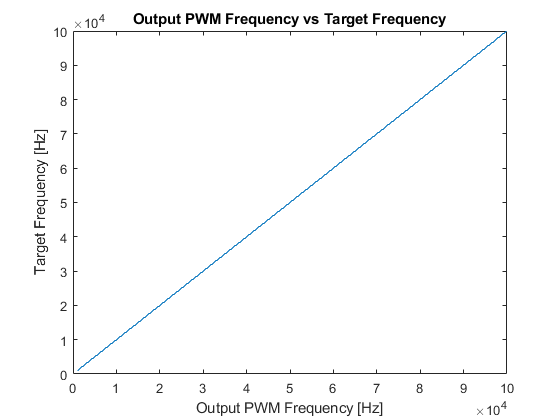
\includegraphics[width=\columnwidth]{pwm/frequency/frequency_range.pdf}
        \subcaption{Output PWM frequency plotted against target frequency}
    \end{subfigure}
    \begin{subfigure}{0.45\textwidth}
        \includegraphics[width=\columnwidth]{pwm/frequency/frequency_error.pdf}
        \subcaption{Output PWM frequency error as a percentage of target frequency}
    \end{subfigure}
    \caption{PWM frequency selection}
    \vspace{-10pt}
    \label{F:pwm_frequency_eval}
\end{figure}

It was also specified that the design would provide a PWM frequency selection error of no more than 200Hz for a provided frequency. This was evaluated numerically by plotting the target output frequency against the systems provided output, and can be seen in \Cref{F:pwm_frequency_eval} (a). To allow for easier visualisation of this error, it was calculated and plotted as a percentage of the target frequency \Cref{F:pwm_frequency_eval} (b). From this data, it was found that the maximum output frequency error of the system was 64Hz, or 0.064\% of the target output.\\

\subsection{PWM Generator Subsystem Evaluation}

The PWM generator subsystem was required to provides a duty cycle selection resolution of at least 1.25\%, and a frequency selection resolution of at least 200Hz, across the 1kHz to 100kHz range. The performed tests show that the implemented subsystem meets these specifications, providing a duty cycle selection resolution of 0.02\%, and a frequency selection resolution of 64Hz.  For the full range of PWM duty cycle and frequency test, measurements, and plots, refer too \Cref{A:digital_PWM}


\section{System State Sensing}\label{S:current_sense_eval}

It was specified in \Cref{S:sensing_design} that a successful state sensing subsystem will provide two sensing elements. The first, an voltage sensor capable of measuring voltages between 3V \& 10V with a resolution of 150mV, specified by requirements 2 \& 3. The second, an inductor current sensor capable of measuring average current and the peak current ripple with a resolution of 15mA, for frequencies between 1kHz \& 100kHz, as specified by requirement 4, 5, 6, \& 7.

\subsection{Output Voltage Sensing}

The design discussed in \Cref{S:v_sense_design} outlines it's capability of measuring a DC voltage between 3V \& 10V, with a measurement resolution of 2.5mV. This measurement precision was evaluated by comparing a selection of known input voltages between 3V and 10V to their measured outputs from the implemented design.\\

From this testing it was identified that a final precision of 10mV was achieved by the design, with signal noise from the ADC presenting as the main design limitation. Although the evaluated resolution of the design does not meet it's designed specification, it still provides a resolution 15 times greater than required.


\subsection{Inductor Current Sensing}

\subsection*{Average Inductor Current}

The design discussed in \Cref{S:avg_current_design} outlines it's capability to provide an average current measurement for frequencies between 1kHz and 100kHz, with a resolution of 244$\mu$A. The frequency range and resolution were evaluated by comparing a selection of known input voltages between 100mV and 3V to their measured outputs from the implemented design. This was then repeated for frequencies of 1kHz, 50kHz, and 100kHz.\\ 

From this testing it was identified that a final precision of 3.5mV was achieved by the design across all frequencies, with similar design limitations as the output voltage sensing. This provided a final average current measurement resolution of 1.1mA.


\subsection*{Peak Inductor Current}

The design discussed in \Cref{S:current_sense_sample_and_hold_design} outlines it's capability to provide a peak current measurement for frequencies between 1kHz and 100kHz, with a resolution of 15mA. As discussed in \Cref{S:peak_current_implementation}, the operation of the original design did not approach the resolution suggested by the simulations, and as such a redesign was undertaken to improve this. 

The precision and functional frequency range of both the initial and final designs were evaluated and compared. In this evaluation, a known peak to peak voltage was input to the design, and compared to it's output DC voltage for a range of frequencies from 1kHz to 100kHz. This was then repeated for input voltages of 150mV, 500mV, and 1500mV, spanning the entire possible input range from the system. An oscilloscope screenshot of this testing for an input of 500mV, and frequencies of 10kHz and 100kHz can be seen in \Cref{F:peak_detect_scope}.

\begin{figure}[H]
    \centering
    \begin{subfigure}{0.45\textwidth}
        \includegraphics[width=\columnwidth]{current_sense/peak_comparison_500mV/10kHz_500mV.PNG}
        \subcaption{Initial (Red) \& final (Blue) peak detetor outputs for a 10$kHz$ 500mV triangle input}
    \end{subfigure}
    \begin{subfigure}{0.45\textwidth}
        \includegraphics[width=\columnwidth]{current_sense/peak_comparison_500mV/100kHz_500mV.PNG}
        \subcaption{Initial (Red) \& final (Blue) peak detetor outputs for a 100$kHz$ 500mV triangle input}
    \end{subfigure}
    \caption{Initial and final peak detector design }
    \vspace{-10pt}
    \label{F:peak_detect_scope}
\end{figure}

From this testing, plots comparing the total error of the two designs as a percentage of the input peak to peak signal were generated, and can be seen in \Cref{F:peak_detect_eval}. From these plots it can be observed that there is an increase in the total error for both designs as the input frequency increases, and a decrease in the total error as the input ripple increases. It can also clearly be seen that the final design provides substantially lower error for all input frequencies and peak to peak values, with a largest recorded error of 8.9\% when operating at the minimum input ripple and maximum frequency.   

\begin{figure}[H]
    \centering
    \begin{subfigure}{0.45\textwidth}
        \includegraphics[width=\columnwidth]{current_sense/error/initial_design_error.pdf}
        \subcaption{Initial design peak current sensing error as a percentage of actual peak current against frequency}
    \end{subfigure}
    \begin{subfigure}{0.45\textwidth}
        \includegraphics[width=\columnwidth]{current_sense/error/final_design_error.pdf}
        \subcaption{Final design peak current sensing error as a percentage of actual peak current against frequency}
    \end{subfigure}
    \caption{Initial and final peak current sensing design, percentage of actual peak current against frequency}
    \vspace{-10pt}
    \label{F:peak_detect_eval}
\end{figure}

From this testing it was identified that a worst case precision of 13.35mV was achieved by the design with an 100kHz input of 150mV peak to peak. After conversion, this provided a worst case peak current measurement resolution of 4.45mA. 

\subsection{State Sensing Subsystem Evaluation}

The state sensing subsystem was required to provide measurements of the buck converters output voltage to a resolution of 150mV, as well as inductor average current and peak current ripple measurements across the 1kHz to 100kHz range to a resolution of 15mA. The performed tests show that the implemented subsystem meets these specifications. This subsystem provides an output voltage measurement resolution of 10mV, an average current sensing resolution of 1.1mA, and a worst case peak ripple sensing resolution of 4.45mA. For the full range of testing, measurements, and plots, refer too \Cref{A:peak_detector}.


\section{Control System}\label{S:control_eval}

It was specified in \Cref{S:control_design} that a successful control subsystem will ensure a steady state error of no more than $\pm$5\% across the output range of 3V to 10V, as specified by requirement 3. It can be noted that the success of this control subsystem relies heavily on the designed specifications of the PWM generator subsystem to implement the selected duty cycle and frequency, as well as the state sensing subsystem to provide reliable and accurate feedback. 

\subsection*{Output Voltage Control}

The design discussed in \Cref{S:output_control_design} outlines it's capability to provide an output steady state error of 23mV, or $\pm$0.78\%. This implemented controller was evaluated using a number of methods, characterising the subsystems steady state error and step response across the across the 3V to 10V output range, as well as the controllers supply change rejection.\\

The step response of the system was evaluated by selecting a system output of 0V DC, and then providing supplying an output target voltage step between 1V DC and 10V DC. From these tests it was observed that there was no output overshoot from the control system, and a consistent settling time of 84ms was observed for all step input values. Oscilloscope screenshots of this controller response can be seen in \Cref{F:control_step}. 

It was also observed from these tests that the designed steady state error of $\pm$0.78\% was achieved, with small output fluctuations of 23mV noticeable in \Cref{F:control_step} (a).

\begin{figure}[H]
    \centering
    \begin{subfigure}{0.45\textwidth}
        \includegraphics[width=\columnwidth]{control/step_response/voltage_control_0-3.PNG}
        \subcaption{Buck converter output voltage controller 3V step response}
    \end{subfigure}
    \begin{subfigure}{0.45\textwidth}
        \includegraphics[width=\columnwidth]{control/step_response/voltage_control_0-10.PNG}
        \subcaption{Buck converter output voltage controller 10V step response}
    \end{subfigure}
    \caption{Buck converter output voltage controller step response for full output voltage range}
    \vspace{-10pt}
    \label{F:control_step}
\end{figure}

The controller response to supply voltage changes was evaluated by allowing the controller to achieve a steady state, and then varying the input supply between values of 6V and 16V respectively. From these tests it was observed that the controller was consistently able to return the output to it's steady state within a period of 250ms. It was also observed that the designed converter was capable of providing any specified output between 1V and 10V across the full tested supply range, so long as the requested output was at least 500mV below the current supply.

\begin{figure}[H]
    \centering
    \begin{subfigure}{0.45\textwidth}
        \includegraphics[width=\columnwidth]{control/variable_input/VCC-step_12-8.PNG}
        \subcaption{Buck converter output voltage controller response to -4V supply transition}
    \end{subfigure}
    \begin{subfigure}{0.45\textwidth}
        \includegraphics[width=\columnwidth]{control/variable_input/VCC-step_8-12.PNG}
        \subcaption{Buck converter output voltage controller response to 4V supply transition}
    \end{subfigure}
    \caption{Buck converter output voltage controller response to varied input supply}
    \vspace{-10pt}
    \label{F:Control_variable_input}
\end{figure}


\subsection{Control Subsystem Evaluation}

The control subsystem was required to ensure that the buck converters output voltage steady state error was no larger than $\pm$5\% across the output range of 3V to 10V. The performed tests show that the implemented sub system meets these specifications. This subsystem has been proven to provide an output voltage steady state error of $\pm$0.78\% across it's full output range, while also providing additional functionality of input supply rejection. This shifts the operating input supply range of all subsystems within this project to between 8V and 16V, as opposed to the static 12V initially specified in requirement 1. 

For the full range of testing, measurements, and plots, refer too \Cref{A:control}.
\chapter{Conclusions}\label{C:conclusion}



%%%%%%%%%%%%%%%%%%%%%%%%%%%%%%%%%%%%%%%%%%%%%%%%%%%%%%%

\backmatter

%%%%%%%%%%%%%%%%%%%%%%%%%%%%%%%%%%%%%%%%%%%%%%%%%%%%%%%

\let\OLDthebibliography\thebibliography
\renewcommand\thebibliography[1]{
  \OLDthebibliography{#1}
  \setlength{\parskip}{0pt}
}

\bibliographystyle{ieeetr}
\bibliography{../../Literature/bibliography}

% Remove the appendix from the table of contents
% \addtocontents{toc}{\protect\setcounter{tocdepth}{-1}}
% \appendix

\chapter*{Acknowledgments}\label{C:ack} 
Thank you Danny B for being great :- ) 

Thank you ECS Techs for putting up with my questions 


\chapter{System Specification Derivation} \label{A:specs}

The system specification derivation equations have been input into the graphing platform \url{Desmos.com}. This has allowed me to visually inspect these equations and form conclusions. The full working and step by step derivation is also available on \url{Desmos.com} using the following links.\\

Duty cycle equation derivation:\\
\url{https://www.desmos.com/calculator/8c7wmbyzw4}\\

Inductor sizing equation derivation:\\ 
\url{https://www.desmos.com/calculator/v7ntrescw5}\\

PWM frequency equation derivation:\\ 
\url{https://www.desmos.com/calculator/ekjhcrt9zg}\\


\chapter{PWM Generation Figures} \label{A:PWM}

\section{Analogue PWM Generation} \label{A:analogue_PWM}


\begin{figure}[H]
    \includegraphics[width = 0.95\textwidth]{pwm/analog/analogue_PWM_ltspice_circuit.png}
    \caption{Analogue PWM LTSpice circuit}
\end{figure}

\begin{figure}[H]
    \includegraphics[width = 0.95\textwidth]{pwm/analog/analogue_PWM_ltspice_1k.png}
    \caption{Analogue PWM LTSpice simulation 1$kHz$}
\end{figure}

\begin{figure}[H]
    \includegraphics[width = 0.95\textwidth]{pwm/analog/analogue_PWM_ltspice_100k.png}
    \caption{Analogue PWM LTSpice simulation 100$kHz$}
\end{figure}


\section{Digital PWM Generation} \label{A:digital_PWM}

\begin{figure}[H]
    \centering
    \begin{subfigure}{0.45\textwidth}
        \includegraphics[width=\columnwidth]{pwm/duty/1kHz_50Duty.JPG}
        \subcaption{Digital PWM Generation at $1kHz$ and a 50\% duty cycle}

    \end{subfigure}
    \begin{subfigure}{0.45\textwidth}
        \includegraphics[width=\columnwidth]{pwm/duty/1kHz_75Duty.JPG}
        \subcaption{Digital PWM Generation at $1kHz$ and a 75\% duty cycle}

    \end{subfigure}
    \caption{Digital PWM Generation at $1kHz$}

\end{figure}

\begin{figure}[H]
    \centering
    \begin{subfigure}{0.45\textwidth}
        \includegraphics[width=\columnwidth]{pwm/duty/100kHz_50Duty.JPG}
        \subcaption{Digital PWM Generation at $100kHz$ and a 50\% duty cycle}

    \end{subfigure}
    \begin{subfigure}{0.45\textwidth}
        \includegraphics[width=\columnwidth]{pwm/duty/100kHz_75Duty.JPG}
        \subcaption{Digital PWM Generation at $100kHz$ and a 75\% duty cycle}

    \end{subfigure}
    \caption{Digital PWM Generation at $100kHz$}

\end{figure}

\chapter{Peak Detector Figures \& Tables}\label{A:peak_detector}

\section*{Precision Rectifier and Sample \& Hold Peak Detector Design Simulations}

\begin{figure}[H]
    \begin{center}
        \includegraphics[width=0.8\textwidth]{current_sense/peak_detection_simulations.png}
        \caption{LTSpice circuit simulation of the precision rectifier and sample and hold peak detection designs.}
    \end{center}
    \vspace{-20pt}
\end{figure}

\section*{Initial \& Final Peak Detector Output Comparison}\label{A:peak_detector_screenshots}

\subsection*{Peak Detector Output for a 150mV Peak to Peak Triangle Input}
\begin{figure}[H]
    
    \centering
    \begin{subfigure}{0.45\textwidth}
        \includegraphics[width=\columnwidth]{current_sense/peak_comparison_150mV/1kHz_150mV.PNG}
        \subcaption{Initial (Red) \& final (Blue) peak detetor outputs for a 1$kHz$ triangle input.}
    \end{subfigure}
    \begin{subfigure}{0.45\textwidth}
        \includegraphics[width=\columnwidth]{current_sense/peak_comparison_150mV/10kHz_150mV.PNG}
        \subcaption{Initial (Red) \& final (Blue) peak detetor outputs for a 10$kHz$ triangle input.}
    \end{subfigure}
    \begin{subfigure}{0.45\textwidth}
        \includegraphics[width=\columnwidth]{current_sense/peak_comparison_150mV/50kHz_150mV.PNG}
        \subcaption{Initial (Red) \& final (Blue) peak detetor outputs for a 50$kHz$ triangle input.}
    \end{subfigure}
    \begin{subfigure}{0.45\textwidth}
        \includegraphics[width=\columnwidth]{current_sense/peak_comparison_150mV/100kHz_150mV.PNG}
        \subcaption{Initial (Red) \& final (Blue) peak detetor outputs for a 100$kHz$ triangle input.}
    \end{subfigure}
    \caption{Initial \& Final Peak Detector Output at varying frequencies for a 150mV peak to peak triangle input.}
\end{figure}

\subsection*{Peak Detector Output for a 500mV Peak to Peak Triangle Input}
\begin{figure}[H]
    
    \centering
    \begin{subfigure}{0.45\textwidth}
        \includegraphics[width=\columnwidth]{current_sense/peak_comparison_500mV/1kHz_500mV.PNG}
        \subcaption{Initial (Red) \& final (Blue) peak detetor outputs for a 1$kHz$ triangle input.}
    \end{subfigure}
    \begin{subfigure}{0.45\textwidth}
        \includegraphics[width=\columnwidth]{current_sense/peak_comparison_500mV/10kHz_500mV.PNG}
        \subcaption{Initial (Red) \& final (Blue) peak detetor outputs for a 10$kHz$ triangle input.}
    \end{subfigure}
    \begin{subfigure}{0.45\textwidth}
        \includegraphics[width=\columnwidth]{current_sense/peak_comparison_500mV/50kHz_500mV.PNG}
        \subcaption{Initial (Red) \& final (Blue) peak detetor outputs for a 50$kHz$ triangle input.}
    \end{subfigure}
    \begin{subfigure}{0.45\textwidth}
        \includegraphics[width=\columnwidth]{current_sense/peak_comparison_500mV/100kHz_500mV.PNG}
        \subcaption{Initial (Red) \& final (Blue) peak detetor outputs for a 100$kHz$ triangle input.}
    \end{subfigure}
    \caption{Initial \& Final Peak Detector Output at varying frequencies for a 500mV peak to peak triangle input.}
\end{figure}

\subsection*{Peak Detector Output for a 1500mV Peak to Peak Triangle Input}
\begin{figure}[H]
    
    \centering
    \begin{subfigure}{0.45\textwidth}
        \includegraphics[width=\columnwidth]{current_sense/peak_comparison_1500mV/1kHz_1500mV.PNG}
        \subcaption{Initial (Red) \& final (Blue) peak detetor outputs for a 1$kHz$ triangle input.}
    \end{subfigure}
    \begin{subfigure}{0.45\textwidth}
        \includegraphics[width=\columnwidth]{current_sense/peak_comparison_1500mV/10kHz_1500mV.PNG}
        \subcaption{Initial (Red) \& final (Blue) peak detetor outputs for a 10$kHz$ triangle input.}
    \end{subfigure}
    \begin{subfigure}{0.45\textwidth}
        \includegraphics[width=\columnwidth]{current_sense/peak_comparison_1500mV/50kHz_1500mV.PNG}
        \subcaption{Initial (Red) \& final (Blue) peak detetor outputs for a 50$kHz$ triangle input.}
    \end{subfigure}
    \begin{subfigure}{0.45\textwidth}
        \includegraphics[width=\columnwidth]{current_sense/peak_comparison_1500mV/100kHz_1500mV.PNG}
        \subcaption{Initial (Red) \& final (Blue) peak detetor outputs for a 100$kHz$ triangle input.}
    \end{subfigure}
    \caption{Initial \& Final Peak Detector Output at varying frequencies for a 1500mV peak to peak triangle input.}
\end{figure}
    

\section*{Initial \& Final Peak Detector Output Error Plots}\label{A:peak_detector_plots}

\begin{figure}[H]
    \begin{center}
        \includegraphics[width=0.8\textwidth]{current_sense/error/150mV_error.pdf}
        \caption{Initial \& final peak detector output error across frequencies for a 150mV peak to peak input. Displayed as a percentage of the ideal output.}
    \end{center}
\end{figure}

\begin{figure}[H]
    \begin{center}
        \includegraphics[width=0.8\textwidth]{current_sense/error/500mV_error.pdf}
        \caption{Initial \& final peak detector output error across frequencies for a 500mV peak to peak input. Displayed as a percentage of the ideal output.}
    \end{center}
    \vspace{-20pt}
\end{figure}

\begin{figure}[H]
    \begin{center}
        \includegraphics[width=0.8\textwidth]{current_sense/error/1500mV_error.pdf}
        \caption{Initial \& final peak detector output error across frequencies for a 1500mV peak to peak input. Displayed as a percentage of the ideal output.}
    \end{center}
\end{figure}


\newpage
\section*{Initial \& Final Peak Detector Output Error Tables}\label{A:peak_detector_tables}


\begin{table}[!ht]
    \centering
    \resizebox{\textwidth}{!}{%
        \begin{tabular}{|l|l|
                >{\columncolor[HTML]{DCFCDC}}l |l|
                >{\columncolor[HTML]{FCDADA}}l |}
            \hline
            \multicolumn{5}{|c|}{\cellcolor[HTML]{FFE4C3}\textbf{\begin{tabular}[c]{@{}c@{}}150mV  Peak to Peak Input Signal\\ Initial and Final Design Peak Detector Output Error Across Frequencies\end{tabular}}}                                                                                     \\ \hline
            \textbf{Frequency (kHz)} & \textbf{Final Design Error (mV)} & \textbf{Final Design \% Error} & \textbf{Initial Design Error (mV)} & \textbf{Initial Design \% Error} \\ \hline
            1                        & -3.90                            & -5.2                           & 3.40                               & 4.533333333                      \\ \hline
            5                        & -3.80                            & -5.066666667                   & 5.80                               & 7.733333333                      \\ \hline
            10                       & -3.70                            & -4.933333333                   & 12.80                              & 17.06666667                      \\ \hline
            15                       & -2.90                            & -3.866666667                   & 18.50                              & 24.66666667                      \\ \hline
            20                       & -2.20                            & -2.933333333                   & 23.30                              & 31.06666667                      \\ \hline
            25                       & -1.60                            & -2.133333333                   & 28.30                              & 37.73333333                      \\ \hline
            30                       & -0.90                            & -1.2                           & 32.60                              & 43.46666667                      \\ \hline
            35                       & -0.30                            & -0.4                           & 36.50                              & 48.66666667                      \\ \hline
            40                       & 0.20                             & 0.266666667                    & 40.20                              & 53.6                             \\ \hline
            45                       & 0.80                             & 1.066666667                    & 43.70                              & 58.26666667                      \\ \hline
            50                       & 1.30                             & 1.733333333                    & 47.00                              & 62.66666667                      \\ \hline
            55                       & 2.00                             & 2.666666667                    & 50.10                              & 66.8                             \\ \hline
            60                       & 2.60                             & 3.466666667                    & 53.00                              & 70.66666667                      \\ \hline
            65                       & 3.10                             & 4.133333333                    & 56.10                              & 74.8                             \\ \hline
            70                       & 3.50                             & 4.666666667                    & 59.50                              & 79.33333333                      \\ \hline
            75                       & 4.00                             & 5.333333333                    & 62.70                              & 83.6                             \\ \hline
            80                       & 4.60                             & 6.133333333                    & 65.20                              & 86.93333333                      \\ \hline
            85                       & 5.00                             & 6.666666667                    & 67.80                              & 90.4                             \\ \hline
            90                       & 5.60                             & 7.466666667                    & 68.10                              & 90.8                             \\ \hline
            95                       & 6.10                             & 8.133333333                    & 68.10                              & 90.8                             \\ \hline
            100                      & 6.70                             & 8.933333333                    & 68.10                              & 90.8                             \\ \hline
        \end{tabular}%
    }
    \caption{Table of output errors at varying frequencies for both the initial and final peak detection design with a 150mV peak to peak input signal.}
    \label{T:150mV_peak_error}
\end{table}


\begin{table}[!ht]
    \centering
    \resizebox{\textwidth}{!}{%
        \begin{tabular}{|l|l|
                >{\columncolor[HTML]{DCFCDC}}l |l|
                >{\columncolor[HTML]{FCDADA}}l |}
            \hline
            \multicolumn{5}{|c|}{\cellcolor[HTML]{FFE4C3}\textbf{\begin{tabular}[c]{@{}c@{}}500mV  Peak to Peak Input Signal\\ Initial and Final Design Peak Detector Output Error Across Frequencies\end{tabular}}}                                                                                     \\ \hline
            \textbf{Frequency (kHz)} & \textbf{Final Design Error (mV)} & \textbf{Final Design \% Error} & \textbf{Initial Design Error (mV)} & \textbf{Initial Design \% Error} \\ \hline
            1                        & -1.60                            & -0.64                          & 7.00                               & 2.8                              \\ \hline
            5                        & -1.70                            & -0.68                          & 15.00                              & 6                                \\ \hline
            10                       & -1.90                            & -0.76                          & 23.90                              & 9.56                             \\ \hline
            15                       & -0.50                            & -0.2                           & 32.90                              & 13.16                            \\ \hline
            20                       & 1.40                             & 0.56                           & 40.70                              & 16.28                            \\ \hline
            25                       & 2.70                             & 1.08                           & 47.90                              & 19.16                            \\ \hline
            30                       & 3.30                             & 1.32                           & 54.40                              & 21.76                            \\ \hline
            35                       & 4.40                             & 1.76                           & 60.60                              & 24.24                            \\ \hline
            40                       & 5.50                             & 2.2                            & 66.30                              & 26.52                            \\ \hline
            45                       & 6.30                             & 2.52                           & 71.90                              & 28.76                            \\ \hline
            50                       & 7.40                             & 2.96                           & 77.30                              & 30.92                            \\ \hline
            55                       & 8.30                             & 3.32                           & 82.40                              & 32.96                            \\ \hline
            60                       & 9.40                             & 3.76                           & 87.40                              & 34.96                            \\ \hline
            65                       & 10.20                            & 4.08                           & 92.50                              & 37                               \\ \hline
            70                       & 11.00                            & 4.4                            & 97.00                              & 38.8                             \\ \hline
            75                       & 11.80                            & 4.72                           & 101.70                             & 40.68                            \\ \hline
            80                       & 12.70                            & 5.08                           & 106.20                             & 42.48                            \\ \hline
            85                       & 13.40                            & 5.36                           & 110.50                             & 44.2                             \\ \hline
            90                       & 14.40                            & 5.76                           & 114.90                             & 45.96                            \\ \hline
            95                       & 15.00                            & 6                              & 119.00                             & 47.6                             \\ \hline
            100                      & 15.80                            & 6.32                           & 123.20                             & 49.28                            \\ \hline
        \end{tabular}%
    }
    \caption{Table of output errors at varying frequencies for both the initial and final peak detection design with a 500mV input signal.}
    \label{T:500mV_peak_error}
\end{table}


\begin{table}[!ht]
    \centering
    \resizebox{\textwidth}{!}{%
        \begin{tabular}{|l|l|
                >{\columncolor[HTML]{DCFCDC}}l |l|
                >{\columncolor[HTML]{FCDADA}}l |}
            \hline
            \multicolumn{5}{|c|}{\cellcolor[HTML]{FFE4C3}\textbf{\begin{tabular}[c]{@{}c@{}}1500mV  Peak to Peak Input Signal\\ Initial and Final Design Peak Detector Output Error Across Frequencies\end{tabular}}}                                                                                     \\ \hline
            \textbf{Frequency (kHz)} & \textbf{Final Design Error (mV)} & \textbf{Final Design \% Error} & \textbf{Initial Design Error (mV)} & \textbf{Initial Design \% Error} \\ \hline
            1                        & 5.40                             & 0.72                           & 15.00                              & 2                                \\ \hline
            5                        & 5.70                             & 0.76                           & 29.70                              & 3.96                             \\ \hline
            10                       & 3.60                             & 0.48                           & 41.70                              & 5.56                             \\ \hline
            15                       & 6.50                             & 0.866666667                    & 55.90                              & 7.453333333                      \\ \hline
            20                       & 9.40                             & 1.253333333                    & 68.70                              & 9.16                             \\ \hline
            25                       & 11.60                            & 1.546666667                    & 79.90                              & 10.65333333                      \\ \hline
            30                       & 13.50                            & 1.8                            & 90.00                              & 12                               \\ \hline
            35                       & 15.10                            & 2.013333333                    & 99.90                              & 13.32                            \\ \hline
            40                       & 17.20                            & 2.293333333                    & 108.70                             & 14.49333333                      \\ \hline
            45                       & 19.20                            & 2.56                           & 117.20                             & 15.62666667                      \\ \hline
            50                       & 20.50                            & 2.733333333                    & 125.50                             & 16.73333333                      \\ \hline
            55                       & 21.90                            & 2.92                           & 133.60                             & 17.81333333                      \\ \hline
            60                       & 23.30                            & 3.106666667                    & 141.50                             & 18.86666667                      \\ \hline
            65                       & 24.80                            & 3.306666667                    & 149.20                             & 19.89333333                      \\ \hline
            70                       & 26.10                            & 3.48                           & 158.20                             & 21.09333333                      \\ \hline
            75                       & 27.50                            & 3.666666667                    & 163.80                             & 21.84                            \\ \hline
            80                       & 28.60                            & 3.813333333                    & 170.70                             & 22.76                            \\ \hline
            85                       & 29.60                            & 3.946666667                    & 177.50                             & 23.66666667                      \\ \hline
            90                       & 30.70                            & 4.093333333                    & 184.40                             & 24.58666667                      \\ \hline
            95                       & 32.10                            & 4.28                           & 191.00                             & 25.46666667                      \\ \hline
            100                      & 33.40                            & 4.453333333                    & 197.50                             & 26.33333333                      \\ \hline
        \end{tabular}%
    }
    \caption{Table of output errors at varying frequencies for both the initial and final peak detection design with a 1500mV input signal.}
    \label{T:1500mV_peak_error}
\end{table}



\chapter{Control System Figures}\label{A:control}
\vspace{-20pt}

\section{Variable Output Voltage Duty Cycle Control} \label{A:control_duty}

\begin{figure}[H]
    
    \centering
    \begin{subfigure}{0.5\textwidth}
        \includegraphics[width=\columnwidth]{control/duty_control/duty_3V.PNG}
        \subcaption{Controlled duty cycle of 28.9\% for a 3V DC output}
    \end{subfigure}
    \begin{subfigure}{0.5\textwidth}
        \includegraphics[width=\columnwidth]{control/duty_control/duty_5V.PNG}
        \subcaption{Controlled duty cycle of 45.25\% for a 5V DC output}
    \end{subfigure}
    \begin{subfigure}{0.5\textwidth}
        \includegraphics[width=\columnwidth]{control/duty_control/duty_10V.PNG}
        \subcaption{Controlled duty cycle of 86.0\% for a 10V DC output}
    \end{subfigure}
    \caption{PWM duty cycle controlled by the voltage output control system (Blue), achieving 3V, 5V and 10V DC (Red).}
\end{figure}

\section{Output Voltage Control Step Response Rise Time} \label{A:control_step_rise}
\begin{figure}[H]
    \centering
    \begin{subfigure}{0.62\textwidth}
        \includegraphics[width=\columnwidth]{control/step_response/voltage_control_0-1.PNG}
        \subcaption{Output voltage controller 0V to 1V step response with 86ms settleing time.}
    \end{subfigure}
    \begin{subfigure}{0.62\textwidth}
        \includegraphics[width=\columnwidth]{control/step_response/voltage_control_0-3.PNG}
        \subcaption{Output voltage controller 0V to 3V step response with 84ms settleing time.}
    \end{subfigure}
    \begin{subfigure}{0.62\textwidth}
        \includegraphics[width=\columnwidth]{control/step_response/voltage_control_0-10.PNG}
        \subcaption{Output voltage controller 0V to 10V step response with 83ms settleing time.}
    \end{subfigure}
    \caption{Output voltage control system step response, reacting to 1V, 3V and 10V output steps.}
\end{figure}

\section{Output Voltage Control Step Response Fall Time} \label{A:control_step_fall}
\begin{figure}[H]
    \centering
    \begin{subfigure}{0.7\textwidth}
        \includegraphics[width=\columnwidth]{control/step_response/voltage_control_3-0.PNG}
        \subcaption{Output voltage controller 3V to 0V step response with 121ms settleing time.}
    \end{subfigure}
    \begin{subfigure}{0.7\textwidth}
        \includegraphics[width=\columnwidth]{control/step_response/voltage_control_10-0.PNG}
        \subcaption{Output voltage controller 10V to 0V step response with 113ms settleing time.}
    \end{subfigure}
    \caption{Output voltage control system step response, reacting to -3V and -10V output steps.}
\end{figure}



\chapter{Schematic \& Printed Circuit Board} \label{A:pcb_and_schematic}

\section{Full System Schematic} \label{A:full_schematic}

\begin{figure}[H]
        \hspace{-65pt}
        \includegraphics[width = 1.3\textwidth]{pcb/buck_converter.pdf}
        \caption{Final system full schematic}

\end{figure}

\section{Designed Printed Circuit Board}

\begin{figure}[H]
    \begin{center}
        \includegraphics[width = 1\textwidth]{pcb/pcb_render.png}
        \caption{Final system printed circuit board rendering}
    \end{center}

\end{figure}


\chapter{Source Code} \label{A:code}

\section*{Single Header Libraries: Hardware Drivers} \label{A:headers}

\subsection*{adc.h} \label{A:adc_code}
\lstinputlisting{code/adc.h} 

\newpage
\subsection*{pid.h} \label{A:pid_code}
\lstinputlisting{code/pid.h}

\newpage
\subsection*{pwm.h} \label{A:pwm_code}
\lstinputlisting{code/pwm.h}

\newpage
\section*{Application Code} \label{A:application_code}

\subsection*{buck\_converter.h}\label{A:buck_code}
\lstinputlisting{code/buck_converter.h} 

\newpage
\subsection*{buck\_converter.c}
\lstinputlisting{code/buck_coverter.c} 

\newpage
\subsection*{main.c} \label{A:main_code}
\lstinputlisting{code/main.c} 


\end{document}
